\documentclass[10pt,letterpaper]{report}
\usepackage[utf8]{inputenc}
\usepackage{amsmath}
\usepackage{amsfonts}
\usepackage{amssymb}
\usepackage{graphicx}
\usepackage{subfig}
\author{Brandon Houghton}
\begin{document}

We observed that there was no explicit grounding of latent features when learning invariants of the data. This can cause learned functions to depend on the random initialization of network weights or bias in sampling of batches. Many useful invariants $\phi^*(x)$ define fundamental parameters of an orbital trajectory and as such can be used to update the state of that trajectory. Thus we used the formulation shown in figure \ref{fig:prednetwork} to drive the latent feature space of the shared network to infer parameters necessary for prediction. This formulation ensures that learned embeddings for $x_t$ encode sufficient information to predict the following state of the orbital trajectory.

Early results yield strong prediction accuracy although learned functions $\phi$ are similar to previous formulations directly predicting $\phi (x_t)$ as seen in figure \ref{fig:overfit}. Overall the new network was prone to over fitting and many hyper parameters resulted in a divergence of the network or a trivial $\phi(x)$ during training as the prediction error dominated the loss function, in the future, pre-training on the prediction network and then introducing a loss function over $\phi$ may produce more consistent results with less need for hyper-parameter tuning. We are continuing to experiment by reducing the size of the latent encoding of orbital parameters to the number of degrees in a 2D orbital trajectory motivated by the concept of the embedding becoming an auto-encoder for the trajectory.


\begin{figure}
	\centering
	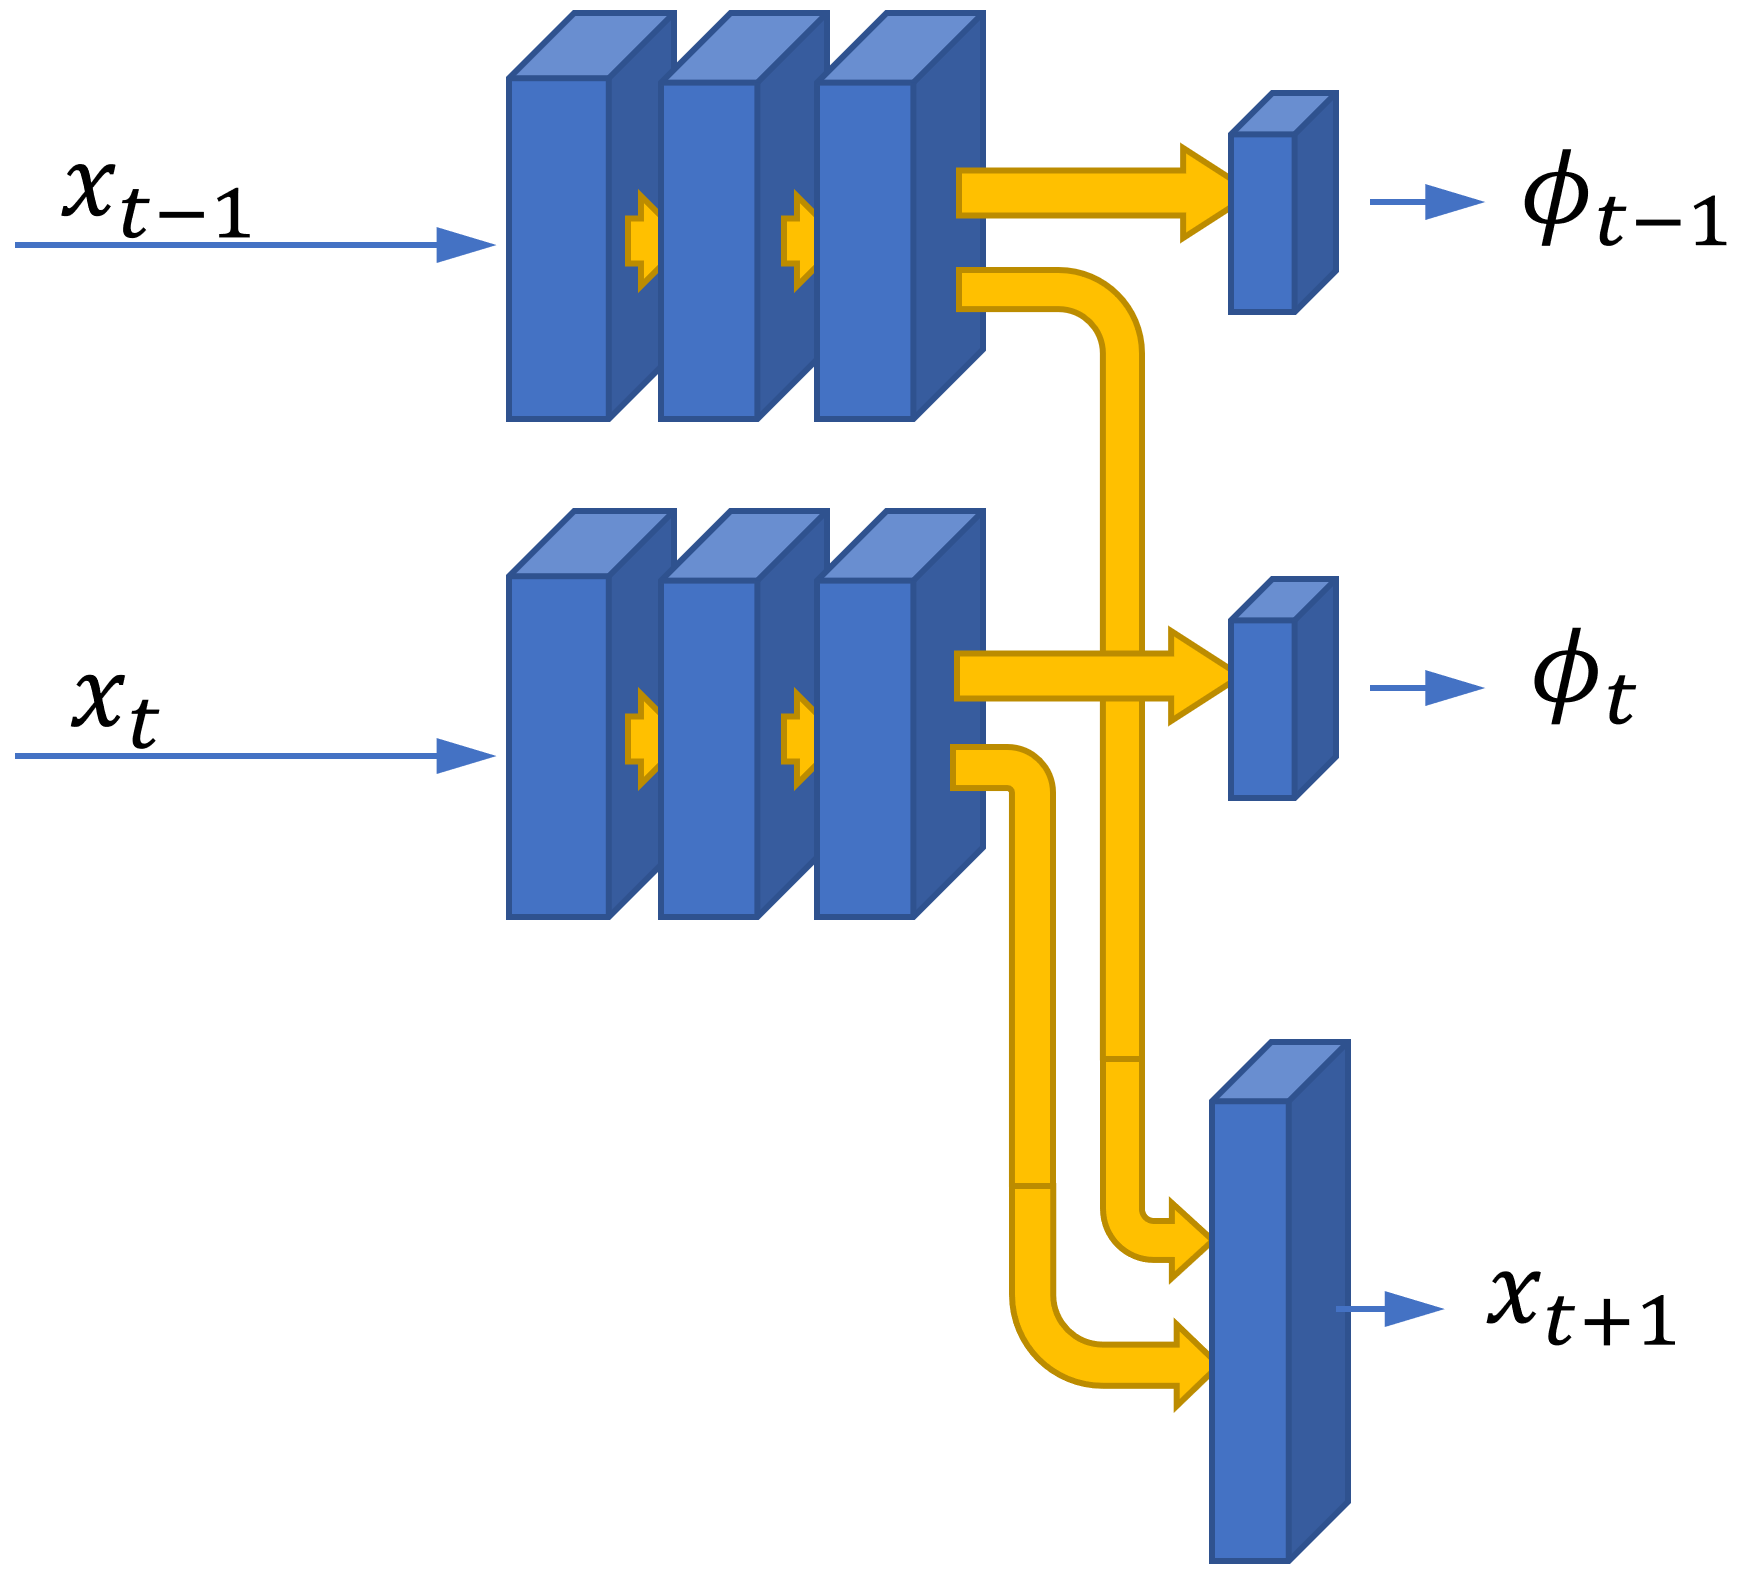
\includegraphics[width=0.7\linewidth]{../images/predNetwork}
	\caption{Using prediction to ground features of discovered invariants}
	\label{fig:prednetwork}
\end{figure}



\begin{figure}%
	\centering
	\qquad
	\subfloat[No prediction loss]{{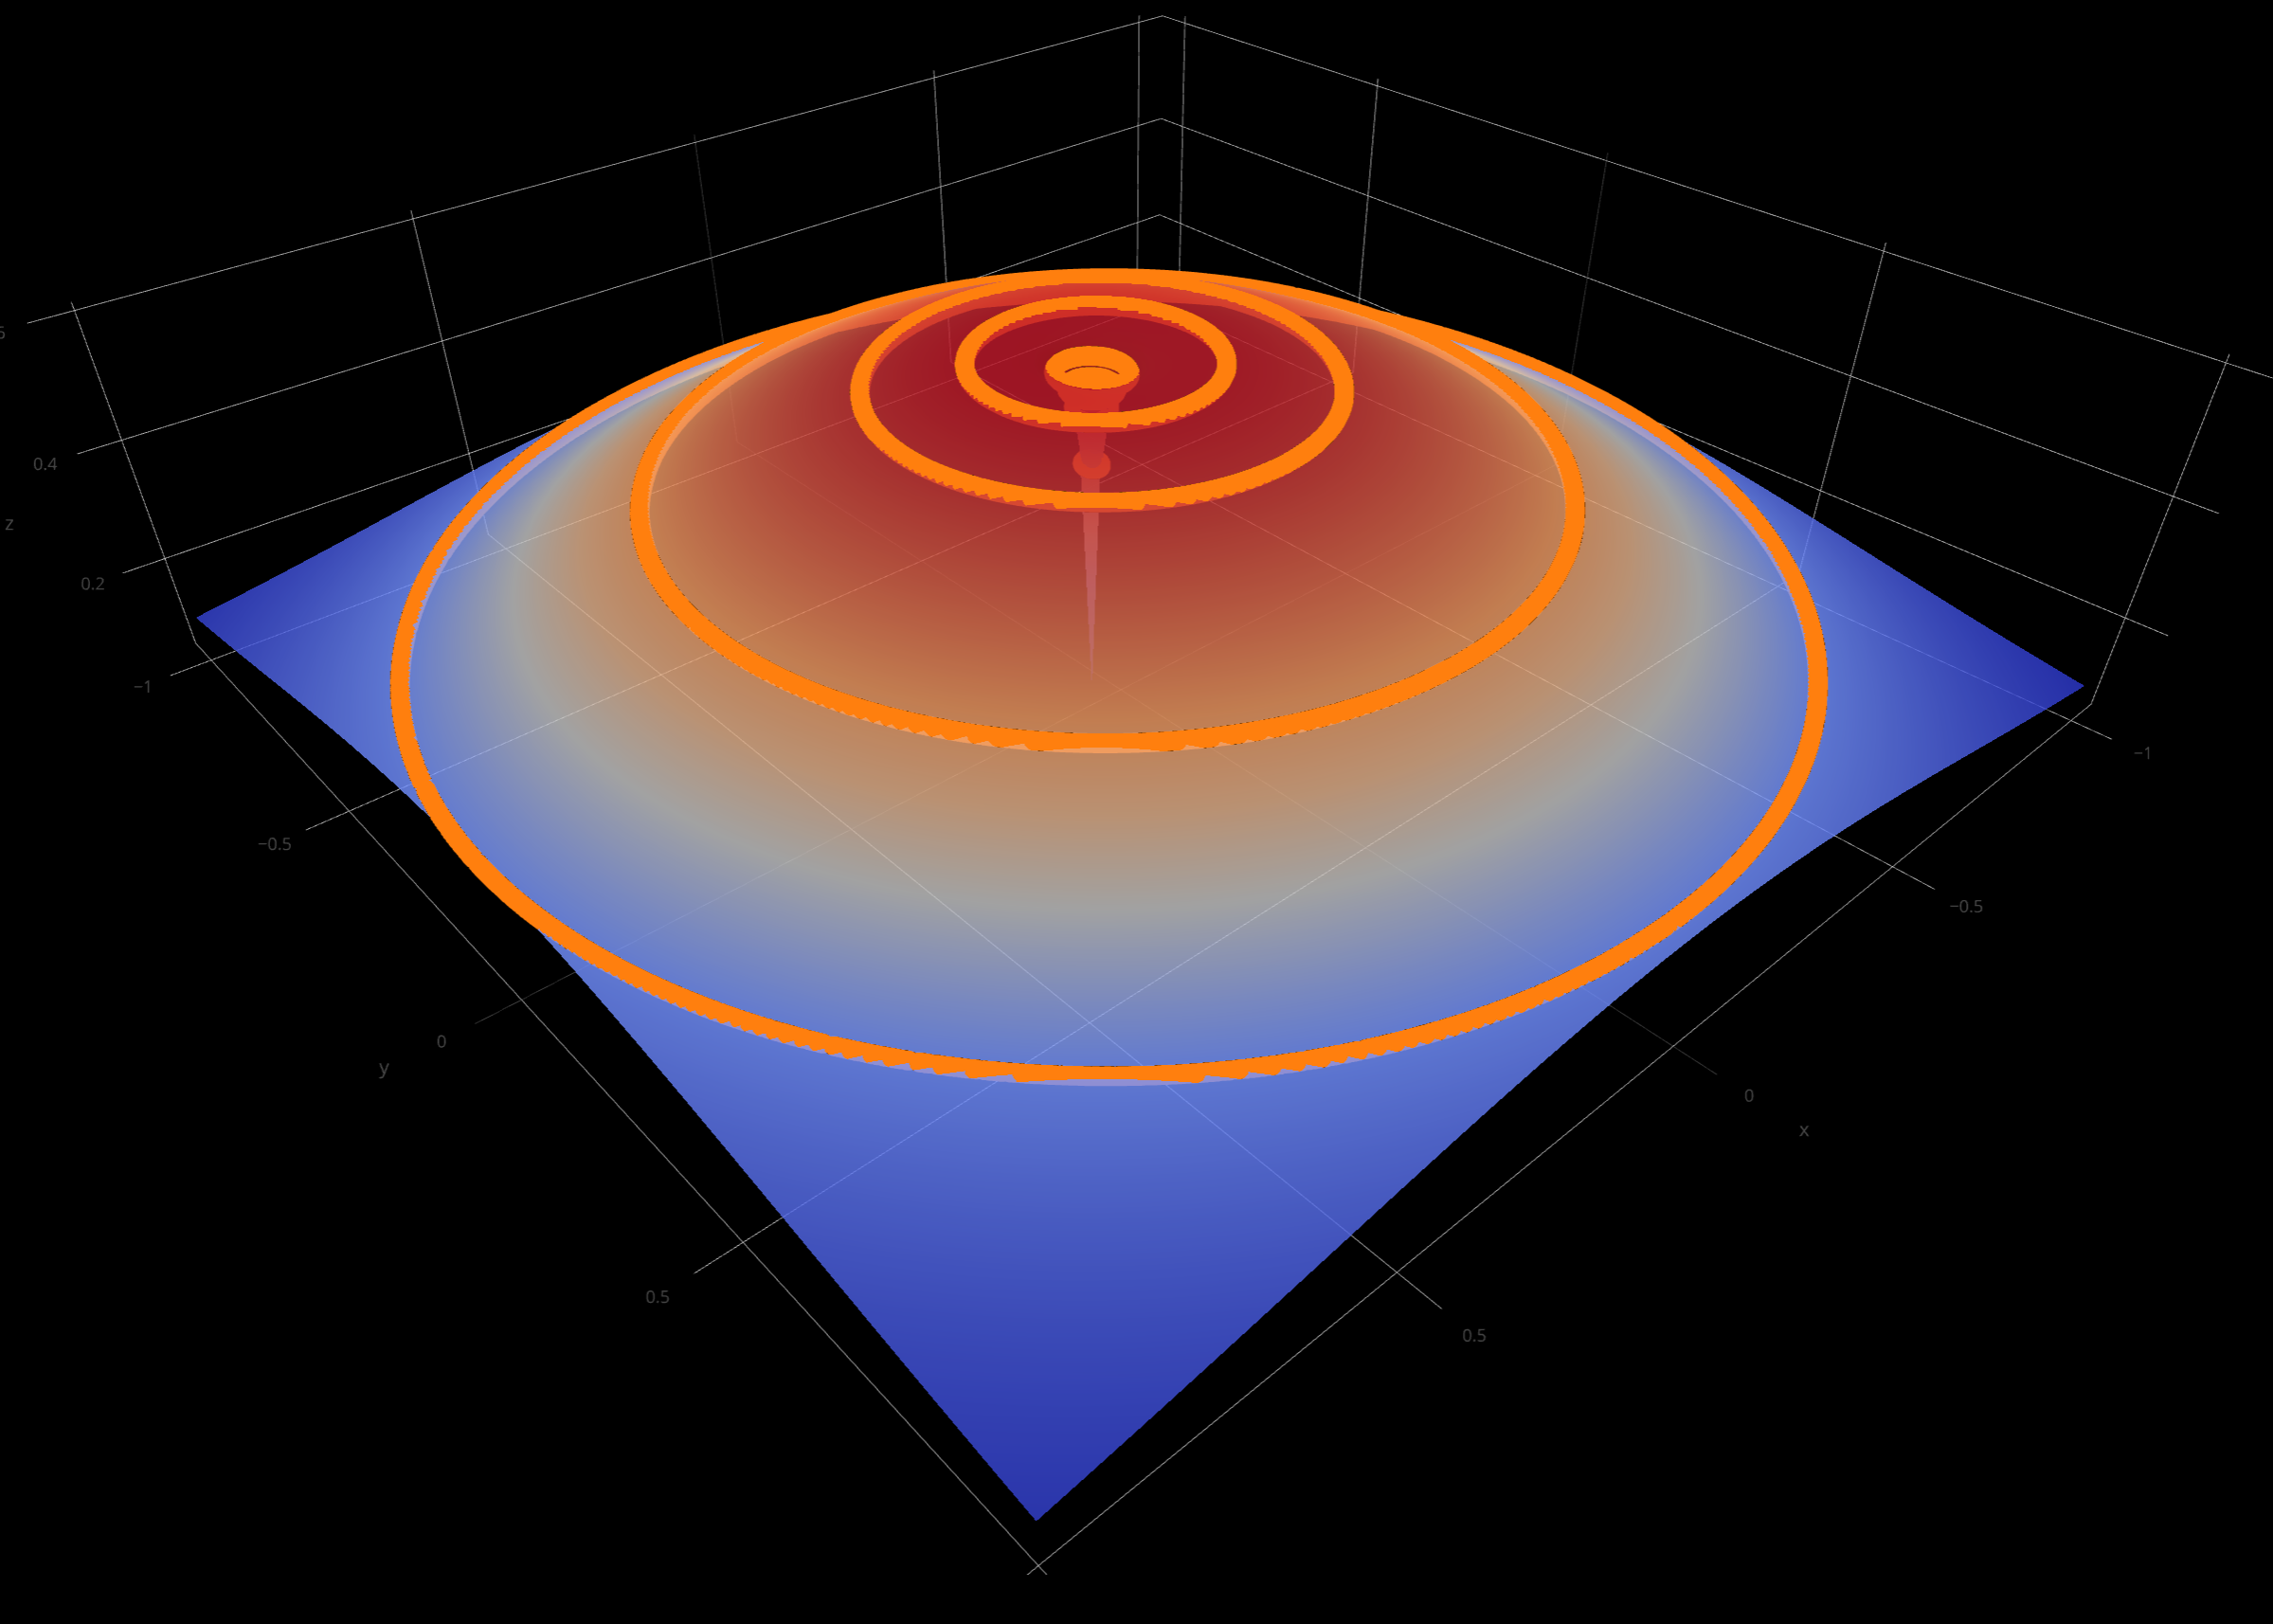
\includegraphics[width=0.41\linewidth]{../images/5000steps}}}%
	\qquad
	\subfloat[With prediction loss]{{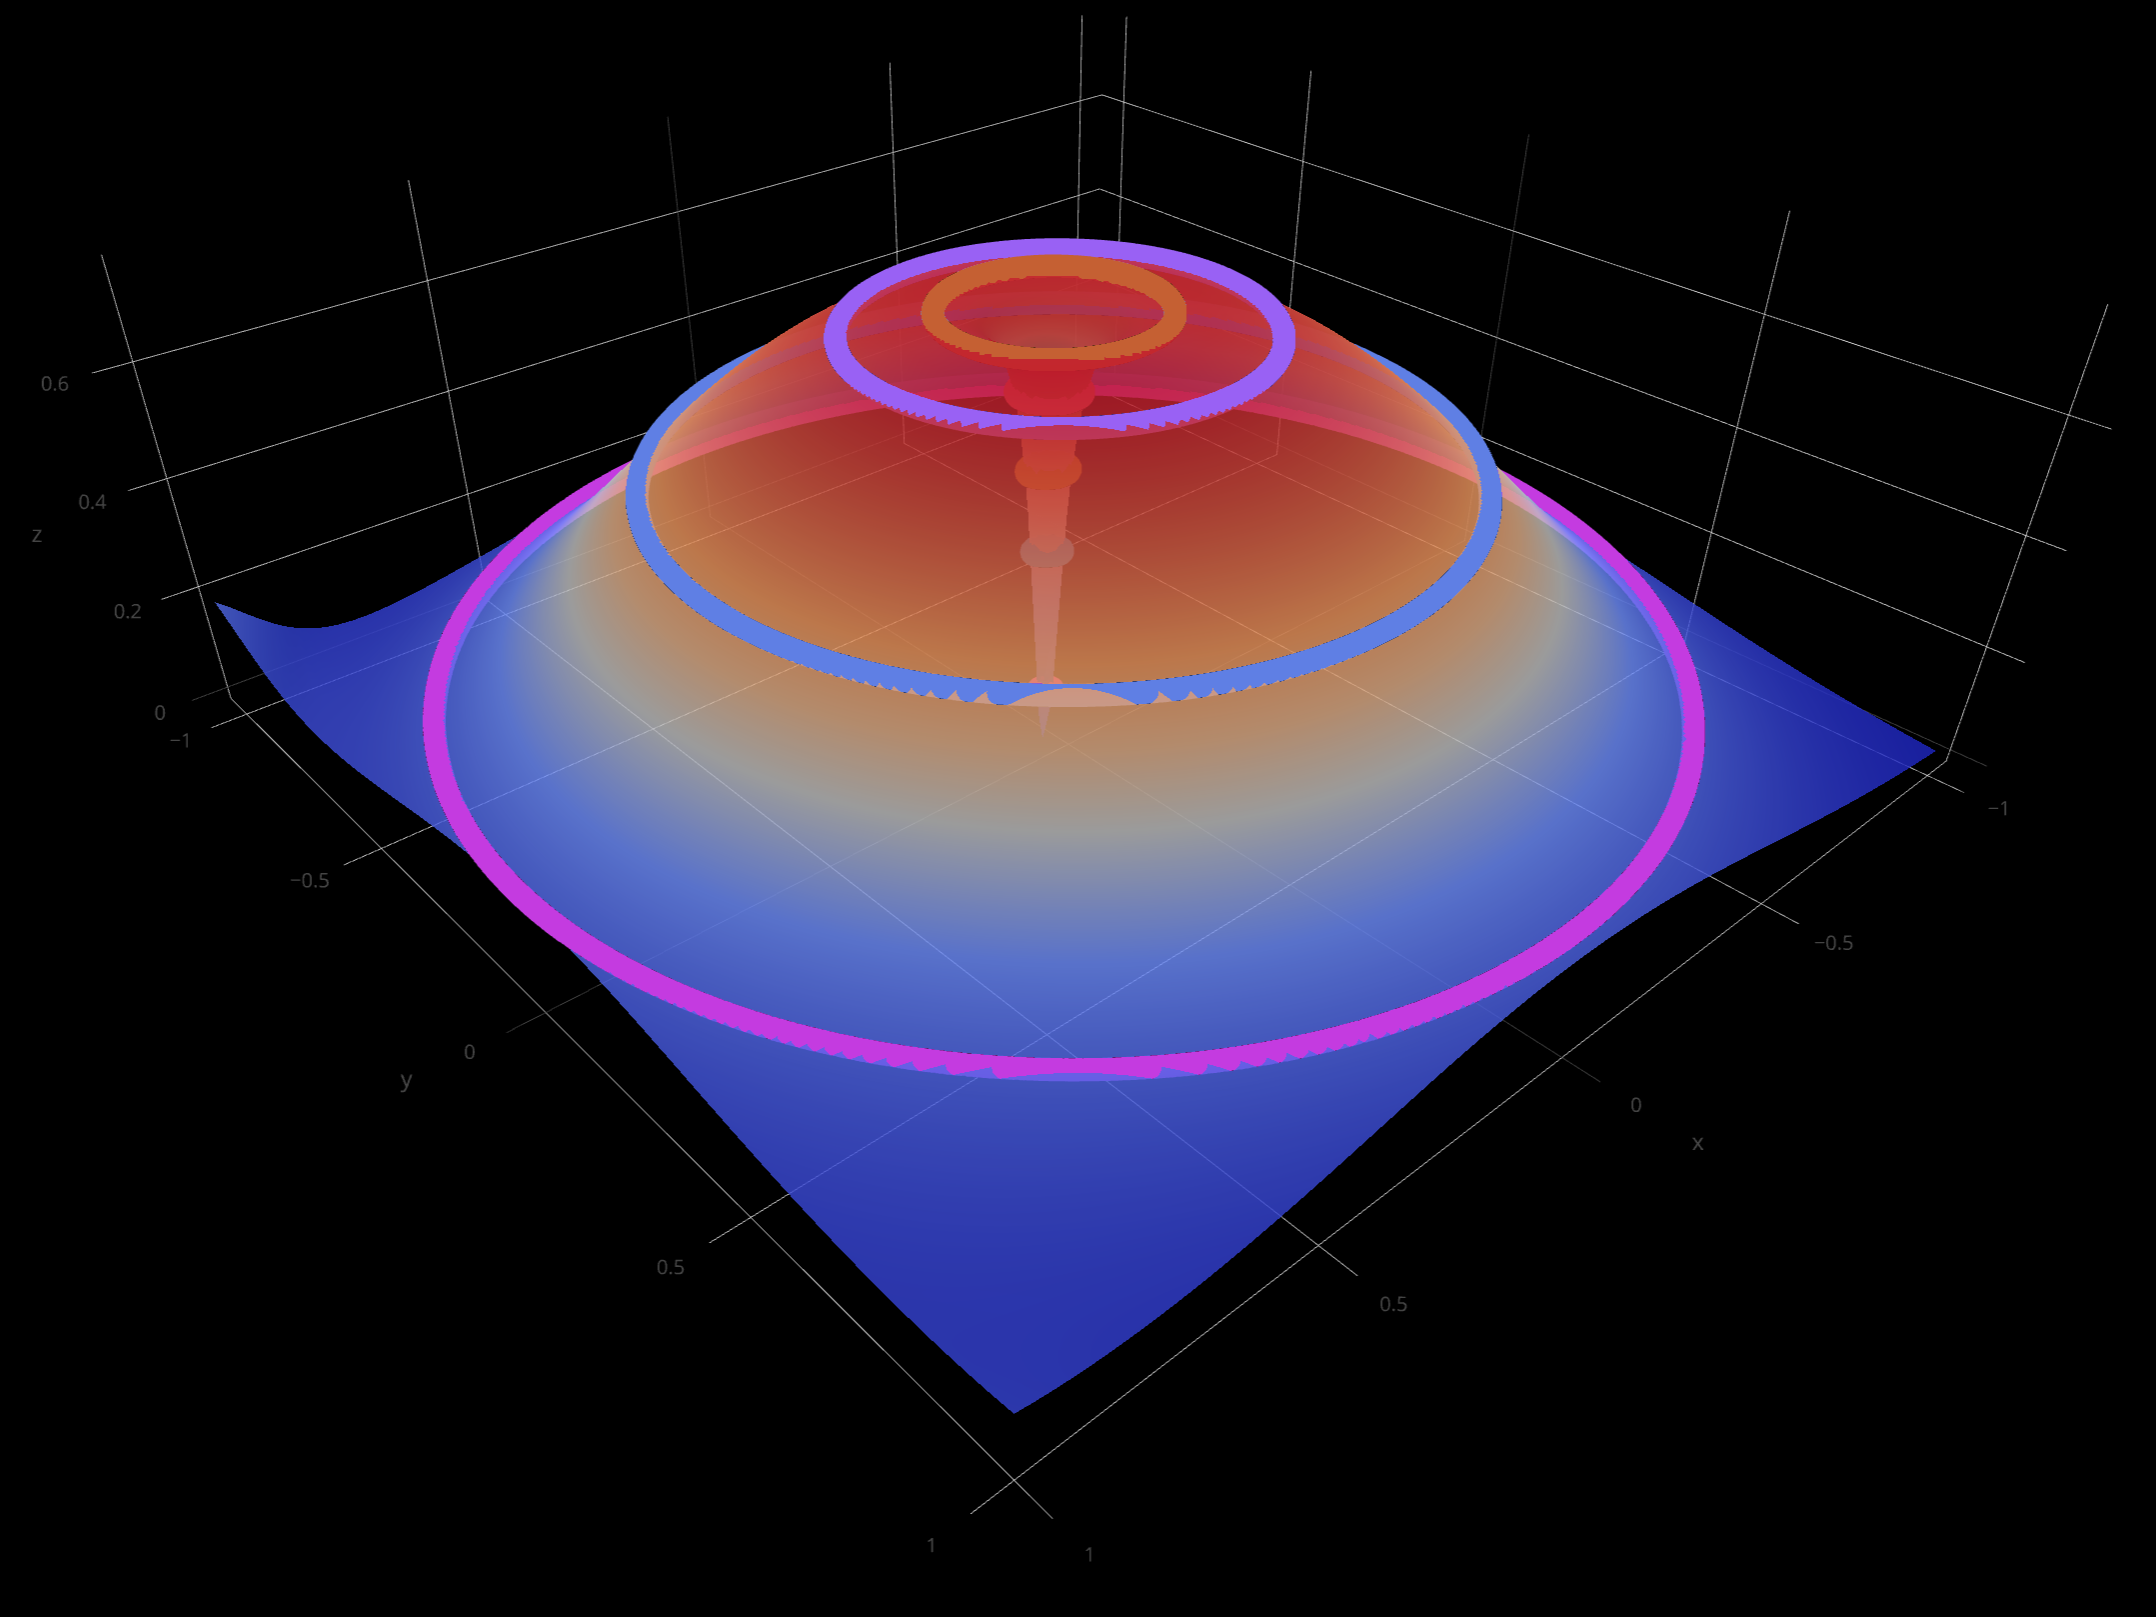
\includegraphics[width=0.41\linewidth]{../images/700steps}}}%
	\caption{Early training results - there seems to be more edge effects when incorporating prediction loss, this may be mitigated by lowering the dimension of the final layer of the shared network }
	\label{fig:overfit}
\end{figure}




\end{document}